%!TEX root = ../lections.tex
Ранее мы рассматривали системы, в которых под действием внешних силовых воздействий появлялись новые режимы. Они являлись неавтономными. Кроме них существует другой тип неавтономных систем и внешнего воздействия. Внешнее воздействие находится внутри системы и может изменять его параметры. Они называются параметрическими, а колебания - параметрическими колебаниями. Пример -- маятник, длина которого периодически меняется, т.е. параметр длины меняется со временем. 

Параметрические системы делят на 2 важных класса: \textbf{резонансные} и \textbf{нерезонансные}. В резонансных системах период изменения параметров находится в целочисленном соотношении с периодом собственных колебаний. В таких системах в такт с изменением энергии, соответствующей собственным колебаниям, вносится энергия, вызванная работой внешнего воздействия. При определенных условиях это может приводить к эффекту раскачки колебаний за счет накапливающейся в системе энергии. Этот эффект лежит в основе работы параметрических усилителей и генераторов. 

К нерезонансным неколебательным параметрическим системам относятся системы, в которых параметры изменяются очень быстро или очень медленно по сравнению с характерным временными масштабами изменения переменных системы. Динамика линейных параметрических систем описывается системой линейных дифференциальных уравнений с периодическими коэффициентами. 

Далее будем рассматривать только линейные параметрические системы. В основе теории таких систем лежит так называемая \textbf{теория Флоке}. 

Рассмотрим двумерную систему
\begin{equation}
	\left\{\begin{aligned}
		&\dot{x_1}=p_{11}(t)\cdot x_1+p_{12}(t)\cdot x_2 \\
		&\dot{x_2}=p_{21}(t)\cdot x_1+p_{22}(t)\cdot x_2,	
	\end{aligned}\right.
	\label{eq:47}
\end{equation}
где $p_{jk}(t+T)=p_{jk}(t)$, то есть  коэффициенты периодически изменяются во времени. Запишем общее решение в матричном виде:
\begin{equation*}
	\vec{x} = X \vec{C}, 
\end{equation*}
где
\begin{gather*}
	\vec{x}= 
	\begin{pmatrix}
		x_1 \\
		x_2
	\end{pmatrix}
	,\quad
	\vec{C}= 
	\begin{pmatrix}
		c_1 \\
		c_2
	\end{pmatrix}
	,\quad
	\vec{X}(t)= 
	\begin{pmatrix}
		\phi_1 ~~  \psi_1 \\
		\phi_2  ~~ \psi_2
	\end{pmatrix}.
\end{gather*}
Здесь векторы
\begin{gather*}
	\vec{\phi}= 
	\begin{pmatrix}
		\phi_1 \\
		\phi_2
	\end{pmatrix}
	,\quad
	\vec{\psi}= 
	\begin{pmatrix}
		\psi_1 \\
		\psi_2
	\end{pmatrix}
\end{gather*}
являются линейно независимыми, следовательно, образуют фундаментальную систему решений. 

Покажем, что в качестве $\phi,\psi$ можно выбрать такие функции, которые удовлетворяют начальным условиям:
\begin{gather}
	\phi_1(0)=1,\quad \psi_1(0)=0, \notag \\ 
	\phi_2(0)=0,\quad \psi_2(0)=1.		
	\label{eq:48}
\end{gather}

Согласно общей теории линейных дифференциальных уравнений вектора $\phi$, $\psi$  будут линейно независимы, если определитель Вронского не обращается в ноль:
\begin{gather*}
	W(t)= 
	\begin{vmatrix}
		\phi_1(t) ~~\psi_1(t) \\ 
		\phi_2(t) ~~\psi_2(t)
	\end{vmatrix}
	,
\end{gather*}
Для ограниченных $W$ верна теорема Лиувилля:
\begin{equation}
	W(t)=W(0)\exp\qty[\int_0^t(p_{11}(t)+p_{22}(t))\dd{t}].
	\label{eq:49}	
\end{equation}

Для начальных условий \eqref{eq:48} получается $W(0)=1$, отсюда следует, что вронскиан отличен от нуля, значит $\phi$, $\psi$ линейно независимы и образуют ФСР.

Поскольку $p_{jk}(t)$ являются периодическими, то вектора $\vec{\phi}(t+T)$, $\vec{\psi}(t+T)$ также линейно не зависимы и являются решением системы \eqref{eq:47}. Как всякое решение, эти вектора можно выразить через ФСР:
\begin{gather}
	\left\{\begin{aligned}
	\vec{\phi}(t+T)=a\vec{\phi}(t)+b\vec{\psi}(t), \\ 
	\vec{\psi}(t+T)=c\vec{\phi}(t)+d\vec{\psi}(t),			
	\end{aligned}\right.
	\label{eq:50}
\end{gather}
где $a,b,c,d$ -- некоторые константы. Их можно найти, подставив $t=0$ и учтя начальные условия \eqref{eq:48}:
\begin{equation}
	a=\phi_1(T),~ b=\phi_2(T),~ c=\psi_1(T),~ d=\psi_2(T).
	\label{eq:51}	
\end{equation}

Соотношения \eqref{eq:51} говорят о том, что константы могут быть найдены, если известно общее решение $\vec\phi, \vec\psi$.

Покажем, что существую такие константы $a,b,c,d$, что для системы  \eqref{eq:47} справедливо:
\begin{equation}
	\vec{x}(t+T)=s\vec{x}(t),
	\label{eq:52}	
\end{equation}
т.е. через период решение повторяется с точностью до множителя.

Поскольку любое решение системы \eqref{eq:47} можно получить из общего решения надлежащим выбором констант, то
\begin{equation}
	\vec{x}(t)=A\vec{\phi}(t)+B\vec{\psi}(t),
	\label{eq:53}	
\end{equation}
% 
% Запишем состояние этого вектора в момент времени $t+T$:
\begin{equation}
	\vec{x}(t+T)=A\vec{\phi}(t+T)+B\vec{\psi}(t+T)
	\label{eq:54}	
\end{equation}
С другой стороны, подставим \eqref{eq:53} и \eqref{eq:54} в \eqref{eq:52}:
\begin{equation}
	A\vec{\phi}(t+T)+B\vec{\psi}(t+T)=s\qty[A\vec{\phi}(t)+B\vec{\psi}(t)].
	\label{eq:55}	
\end{equation}
Теперь используем \eqref{eq:50}:
\begin{equation}
	\qty[A(a-s)+Bc]\vec{\phi}(t)+\qty[Ab+B(d-s)]\vec{\psi}(t) \equiv 0.
	\label{eq:56}	
\end{equation}
Для выполнения равенства при любом $t$ нужно, чтобы скобки с коэффициентами обратились в ноль:
\begin{equation}
	\left\{\begin{aligned}
		&A(a-s)+Bc=0 \\
		&Ab+B(d-s)=0.		
	\end{aligned}\right.
	\label{eq:57}
\end{equation}
Это СЛАУ относительно коэффициентов $A$, $B$. Раскрываем определитель:
\begin{equation}
	s^2-(a+d)s+ad-bc=0.
	\label{eq:58}	
\end{equation}
Оказывается, что $ad-bc$ всегда можно найти, не находя общего решения.

Вернемся к вронскиану. Подсчитаем его в момент времени $T$:
\begin{gather*}
	W(T)= 
	\begin{vmatrix}
		\phi_1(T) & \psi_1(T) \\ 
		\phi_2(T) & \psi_2(T)
	\end{vmatrix}
	=
	\begin{vmatrix}
		a & c \\ 
		b & d
	\end{vmatrix}
	=ad-bc.
\end{gather*}
с другой стороны,
\begin{eqnarray*}
	W(T)=\underbrace{W(0)}_{\text{=1}}\exp\qty[\int_0^T(p_{11}(t)+p_{22}(t))\dd{t}] \\
\end{eqnarray*}
\begin{equation}
	ad-bc=\exp\qty[\int_0^T\qty(p_{11}(t)+p_{22}(t))\dd{t}].
	\label{eq:59}
\end{equation}
Так как $p_{11}, p_{22}$ мы знаем из постановки конкретной задачи, то $ad-bc$ всегда найдём.

Предположим, что \eqref{eq:58} не имеет кратных корней, следовательно, существует два значения мультипликатора и два решения:
\begin{gather}
	\vec{x}_1(t+T)=s_1\vec{x}_1(t) \notag \\ 
	\vec{x}_2(t+T)=s_2\vec{x}_2(t).		
	\label{eq:60}
\end{gather}
Таким образом, решение воспроизводит себя через период с точностью до множителя. 
\begin{gather}
	\vec{x}_1(t+nT)=(s_1)^n\vec{x}_1(t) \notag \\ 
	\vec{x}_2(t+nT)=(s_2)^n\vec{x}_2(t).		
	\label{eq:61}
\end{gather}

Покажем, что решения $\vec{x}_1,\vec{x}_2$ можно представить в следующем виде:
\begin{gather}
	\vec{x}_1(t)=e^{\lambda_1t}\vec{\Phi}_1(t), \qquad
	\vec{x}_2(t)=e^{\lambda_2t}\vec{\Phi}_2(t),		
	\label{eq:62}
\end{gather}
где $\lambda$ -- некоторые числа, которые называются характеристическими, а вектора $\Phi$ имеют вид
\begin{gather*}
	\vec{\Phi}_1(t)= 
	\begin{pmatrix}
		\Phi_{11} \\
		\Phi_{21}
	\end{pmatrix}
	,\quad
	\vec{\Phi}_2(t)= 
	\begin{pmatrix}
		\Phi_{12} \\
		\Phi_{22}
	\end{pmatrix}
	,
\end{gather*}
и являются периодическими с периодом $T$:
\begin{equation}
	\Phi_{jk}(t+T)=\Phi_{jk}(t),
	\label{eq:63}
\end{equation}
а характеристические числа представляются в следующем виде:
\begin{gather}
	\lambda_j=\frac{1}{T}\,\mathrm{Ln}\,s_j=\frac1{T}\qty[\vphantom{\bigg|}\ln|s_j|\pm i\qty(\vphantom{\big|}\arg s_j +2\pi k)], \quad
	\begin{aligned}
		&j=1,2, \\
		&k=0,\pm 1, \pm 2, \ldots	
	\end{aligned}
	\label{eq:64}
\end{gather}
$s$ -- мультипликаторы, которые могут быть комплексными, поэтому присутствует аргумент комплексного числа.

Покажем справедливость \eqref{eq:63}. Из \eqref{eq:62}:
\begin{equation*}
	\vec{\Phi}_j(t)=e^{-\lambda_j t}\vec{x}_j(t),
\end{equation*}
но $\vec{x}_j$ можно выразить из \eqref{eq:60}:
\begin{gather*}
	\vec{x}_j(t+T)=s\vec{x}_j(t)=e^{\lambda_0 T}\vec{x}_j(t), \\
	\vec{\Phi}_j(t+T)=e^{-\lambda_0(t+T)}\vec{x}_j(t+T)=e^{\lambda_0 T}\vec{x}_j(t)e^{-\lambda_j(t+T)}=\vec{x}_j(t)e^{-\lambda_j t}=\vec{\Phi}_j(t).
\end{gather*}

С другой стороны, $\vec{x}_j$ образуют ФСР, поэтому общее решение можно записать в виде
\begin{equation}
	\vec{x}_j(t)=\sum_{j=1}^2 c_j e^{\lambda_j t}\vec{\Phi}_j(t).
	\label{eq:65}
\end{equation}

Это основное соотношение ЛДУ с переменными параметрами. Здесь $\Phi$ -- функции Флоке. 

\paragraph{Замечание. } Теория Флоке может быть применена к предельным циклам, так как  они являются переодическим решением. 




\subsection{Отображение через период}

С точки зрения теории динамических систем, \eqref{eq:47} представляет собой неавтономную систему, следовательно, порождает точечное отображение $$g^t:\mathds{R}^2\rightarrow \mathds{R}^2.$$
\begin{figure}[H]
	\centering
	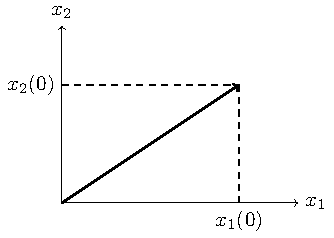
\includegraphics[width=0.35\linewidth]{fig/fig33.pdf}   
\end{figure}

Под действием системы \eqref{eq:47} вектор $\vec{x}(0)$ переходит в другой вектор $\vec{v}(t)$:
\begin{equation*}
	g^t\vec{x}(0)=\vec{v}(t).
\end{equation*}
если $t=0: \vec{x}(0)=\vec{v}(0)$.
В силу теории Флоке наибольший интерес представляет отображение через период, т.е. $g^T$. Заметим, что решение $x_1=0, x_2=0$ является неподвижной точкой этого отображения. Более того, с точки зрения неавтономной системы, это периодическое решение любого периода. 

Воспользуемся соотношением Флоке:
\begin{gather}
	x_1(t)=C_1 e^{\lambda_1 t}\Phi_{11}(t)+C_2 e^{\lambda_2 t}\Phi_{12}(t) \notag \\ 
	x_2(t)=C_1 e^{\lambda_1 t}\Phi_{21}(t)+C_2 e^{\lambda_2 t}\Phi_{22}(t).	
	\label{eq:66}
\end{gather}
Пусть $x_1(0)=x_1$, $x_2(0)=x_2$. Подставим $t=0$ в \eqref{eq:66}, находим $C_1^0, C_2^0$ через получившуюся СЛАУ. 
% Задаем точку, находим ее образ через период:
% \begin{gather}
% 	x_1(t)=C_1^0 e^{\lambda_1 t}\Phi_{11}(t)+C_2^0 e^{\lambda_2 t}\Phi_{12}(t) \notag \\ 
% 	x_2(t)=C_1^0 e^{\lambda_1 t}\Phi_{21}(t)+C_2^0 e^{\lambda_2 t}\Phi_{22}(t),		
% 	\label{eq:67}
% \end{gather}

Используя \eqref{eq:53}, а также связь A и B с a, b, c, d:
\begin{gather*}
	\Phi_{11}(0)=A_1,~\Phi_{12}(0)=A_2,~\Phi_{21}(0)=B_1,~\Phi_{22}(0)=A_2.	
\end{gather*}
\begin{equation}
	g^T\rightarrow
	\left\{\begin{aligned}
		x_1(T)=a x_1(0)+c x_2(0) \\
		x_2(T)=b x_1(0)+d x_2(0)		
	\end{aligned}\right.
	\label{eq:68}
\end{equation}
\begin{gather*}
	\vec{x}(T)=G \vec{X}(0),~ G=
	\begin{pmatrix}
		a ~b \\
		c ~d \\
	\end{pmatrix}
	,\\
	a=\phi_1(T), ~ b=\phi_2(T), \\
	c=\psi_1(T), ~ d=\psi_2(T).
\end{gather*}

Траектории системы порождают порождают точечное отображение. Роль дискрета играет период T. Отображение линейное. Нужно исследовать устойчивость неподвижных точек. 
\subsection{Устойчивость нулевого решения}
Вспомним точечное отображение. Поведение $g^T$ зависит от мультипликаторов.

Пусть $s_1, s_2$ - действительные. Тогда \eqref{eq:68} с помощью преобразования можно привести к виду:
\begin{equation*}
	\left\{\begin{aligned}
		U_1(T)=s_1 U_1(0) \\
		U_2(T)=s_2 U_2(0)		
	\end{aligned}\right.
\end{equation*}
\begin{enumerate} 
	\item Поскольку мультипликаторы $s_1, s_2$ соответствуют решениям неавтономной \eqref{eq:47} системы, они удовлетворяют условию $s_1\cdot s_2>0$;
	\item Если $|s_j|<1$, неподвижная точка устойчива, если $|s_j|>1$ - неустойчива. Если $|s_i|<1, |s_j|>1, s_i \neq s_j$, то точка - седло. 
\end{enumerate} 

Пусть $0<s_j<1$:
\begin{figure}[H]
	\centering
	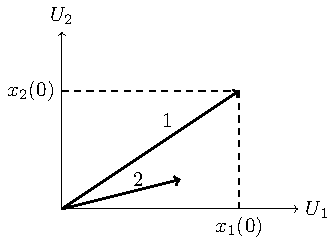
\includegraphics[width=0.35\linewidth]{fig/fig34.pdf}   
\end{figure}

Вектор уменьшит длину и повернется. Любое начальное условие стремится к нулю, следовательно, решение устойчивое.

$-1<s_j<0$:
\begin{figure}[H]
	\centering
	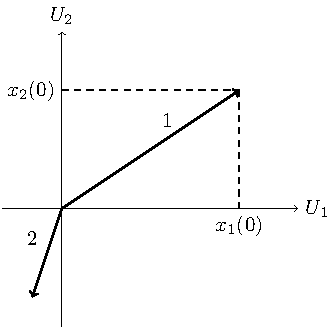
\includegraphics[width=0.35\linewidth]{fig/fig35.pdf}   
\end{figure}

Вектор уменьшит длину и переместится в отрицательную область. Будут скачки. Решение устойчиво.

$0<|s_1|<1, |s_2|>1$:
\begin{figure}[H]
	\centering
	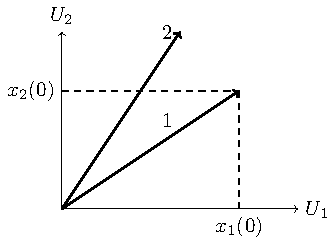
\includegraphics[width=0.35\linewidth]{fig/fig36.pdf}   
\end{figure}

По одной координате растяжение, а по другой сжатие. Вектор асимптотически прижимается к оси ординат.

$-1<|s_1|<0, |s_2|<-1$:
\begin{figure}[H]
	\centering
	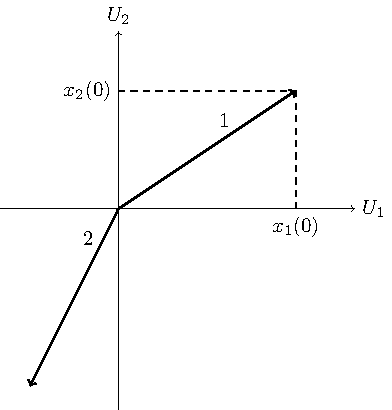
\includegraphics[width=0.35\linewidth]{fig/fig37.pdf}   
\end{figure}

Вектор прижимается к оси координат и растягивается.

29.04

Рассмотрим комплексно-сопряженные корни. Линейным преобразованием систему можно привести к нормальной форме.
\begin{equation}
	U_j(T)=s_j U_j(0), ~j=1,2.
	\label{eq:69}
\end{equation}

$|s|<1$ - длина вектора меняется.
\begin{equation}
	s_j=\alpha \pm i\beta.
	\label{eq:70}
\end{equation}
Поскольку мультипликаторы являются комплексно сопряженными, переменные $U_j(T), U_j(0)$ являются комплексными функциями. 
\begin{gather}
	U_j(0)=U(0)\pm iV(0) \notag \\ 
	U_j(T)=U(T)\pm iV(T).		
	\label{eq:71}
\end{gather}

Подставляя \eqref{eq:70}, \eqref{eq:71} в \eqref{eq:69} и разделяя реальную и мнимую части, получим:
\begin{gather}
	U(T)=\alpha U(0)- \beta V(0) \notag \\ 
	V(T)=\beta U(0)+ \alpha V(0).		
	\label{eq:72}
\end{gather}
\begin{gather*}
	U=\rho \cos{\phi}, V=\rho \sin{\phi}, \\ 
	s=\alpha \pm i\beta=|s|e^{\pm i \omega}, \\
	|s|=\sqrt{\alpha^2+\beta^2},		
\end{gather*}
\begin{gather}
	\alpha=|s|\cos{\omega} \notag \\ 
	\beta=|s|\sin{\omega}.		
	\label{eq:73}
\end{gather}
\begin{equation}
	\left\{\begin{aligned}
		\rho(T)\cos{\phi(T)}=\alpha \rho(0)\cos{\phi(0)}-\beta \rho(0)\sin{\phi(0)} \\
		\rho(T)\sin{\phi(T)}=\beta \rho(0)\cos{\phi(0)}+\alpha \rho(0)\sin{\phi(0)}.
	\end{aligned}\right.
	\label{eq:74}
\end{equation}
Из этой системы находят $\rho(T)$ и $\phi(T)$:
\begin{equation}
	\left\{\begin{aligned}
		\phi(T)=\phi(0)+\omega \\
		\rho(T)=|s|\rho(0).
	\end{aligned}\right.
	\label{eq:75}
\end{equation}

Эта система задает отображение $g^T$. Полярный угол $\phi$ меняется за период на $\omega$, а начальная величина вектора $\rho(0)$ изменяется в зависимости от s. 

Если $|s|<1$:
\begin{figure}[H]
	\centering
	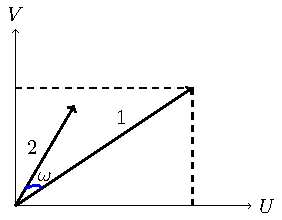
\includegraphics[width=0.35\linewidth]{fig/fig38.pdf}   
\end{figure}

Вектор поворачивается на угол $\omega$ и сокращается в длину. Состояние равновесия и соответствующая ему неподвижная точка $x_1=x_2=0$ являются асимптотически устойчивыми.

$|s|>1$:
\begin{figure}[H]
	\centering
	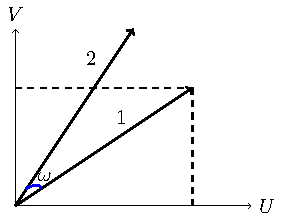
\includegraphics[width=0.35\linewidth]{fig/fig39.pdf}   
\end{figure}

Состояние равновесия неустойчивое, вектор поворачивается и растягивается.

$|s|=1$:
\begin{figure}[H]
	\centering
	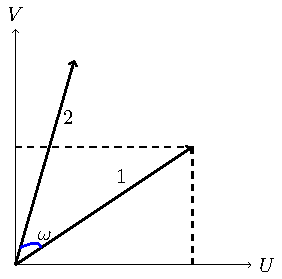
\includegraphics[width=0.35\linewidth]{fig/fig40.pdf}   
\end{figure}

Вектор поворачивается, длина его не меняется. 

Вектор, пройдя период, может либо совпасть с начальным, либо нет. В зависимости от этого решение будет периодическим или квазипериодическим.

Таким образом, состояние равновесия или периодическая траектория любого периода в параметрической системе может быть устойчивой либо не устойчивой.

\subsection{Основные режимы линейной параметрической системы}

Поскольку система линейная, из условия устойчивости состояния равновесия вытекают все остальные свойства линейных параметрических систем, а именно:
\begin{enumerate} 
	\item Параметрическая система, находящаяся в начальный момент в состоянии равновесия, останется в этом состоянии при $\forall t>0$, поскольку состояние равновесия $x_1=x_2=0$ существует всегда в линейной системе. Параметрическую систему, находящуюся в состоянии равновесия, нельзя вывести из этого состояния, изменяя ее параметры. Пример - маятник на нитке: дергая за нитку, маятник нельзя раскачать;
	\item Состояние равновесия параметрической системы может быть как устойчивым, так и не устойчивым;
	\item Если параметры системы таковы, что она неустойчива и система выведена из состояния равновесия, то в ней возникают колебания, амплитуда которых экспоненциально возрастает. Этот процесс возрастания размахов колебаний при периодическом нарастании колебаний, называется параметрическим резонансом.
\end{enumerate} 

\subsection{Параметрические колебания. Резонанс.}
Установим условие существования параметрического резонанса в одном частном, но важном случае. Рассмотрим систему \eqref{eq:47} в случае $p_{11}(t) \equiv0, p_{12}(t)\equiv 1, p_{22}(t) \equiv 0$, тогда система примет вид:
\begin{equation}
	\left\{\begin{aligned}
		\dot{x_1}=x_2 \\
		\dot{x_2}=p_{21}(t)x_1.
	\end{aligned}\right.
	\label{eq:76}
\end{equation}

Система \eqref{eq:76} охватывает уравнения Матье и Хилла. 

Поведение системы определяют мультипликаторы, а они, в свою очередь, определяются характеристическим уравнением:
\begin{gather*}
	s^2-(a+d)s+(ad-bc)=0, \\
	ad-bc=exp\qty[\int_0^T(p_{11}(t)+p_{22}(t))\dd{t}]=1.		
\end{gather*}

Фактически, варьируются только коэффициенты a и d. Введем: $2P=a+d$ - контрольный параметр.
\begin{gather*}
	s^2-2Ps+1=0.		
\end{gather*}

Проанализируем поведение s.
Пусть $|P|<1$
\begin{gather*}
	s_{1,2}=P\pm i\sqrt{1-P^2}, \\
	|s|=1.		
\end{gather*}

Неподвижная точка отображения $g^T$ будет эллиптической. 

Достаточно рассмотреть только $x_1(t)$:
\begin{equation}
	x_1(t)=c_1e^{\lambda_1 t}\Phi_{11}(t)+c_2e^{\lambda_2 t}\Phi_{12}(t).
	\label{eq:77}
\end{equation}

Поскольку $|s|=1$, характеристические показатели $\lambda$ связаны с s: $\lambda_1=\frac{q}{T}i,~\lambda_2=-\frac{q}{T}i$, где $q=|arg(s_j)+2\pi k|$ (из формулы \eqref{eq:64}). $\lambda$ чисто мнимые, x действительные, следовательно, $c_1, c_2, \Phi_{11}, \Phi_{12}$ должны быть комплексными:
\begin{equation}
	\left\{\begin{aligned}
		c_1=\frac{A}{2}e^{ic} \\
		c_2=\frac{A}{2}e^{-ic} \\
		\Phi_{11}=h(t)e^{i\varkappa(t)} \\
		\Phi_{12}=h(t)e^{-i\varkappa(t)}.
	\end{aligned}\right.
	\label{eq:78}
\end{equation}

Подставляя \eqref{eq:78} в \eqref{eq:77}, получим:
\begin{equation}
	x_1(t)=Ah(t)\cos (\frac{q}{T}t+c+\varkappa(t)).
	\label{eq:79}
\end{equation}

Вспомним косинус суммы, чтобы выделить соответственные временные масштабы. $h(t)$ и $\varkappa(t)$ периодичны с периодом T (из теории Флоке). T - период изменения параметров.
\begin{equation}
	x_1(t)=H(t)\cos{(\frac{q}{T}t+c)}+F(t)\sin{(\frac{q}{T}t+c)}.
	\label{eq:80}
\end{equation}
\begin{gather*}
	H(t)=Ah(t)\cos \varkappa(t), \\
	F(t)=-Ah(t)\sin \varkappa(t).		
\end{gather*}

В \eqref{eq:80} $H(t)$ и $F(t)$ периодичны с периодом T. Есть два временных масштаба: $T_1=T$ и $T_2=\frac{2\pi}{q}T$, которым отвечают частоты $\omega_1$ и $\omega_2$ соответственно.

$\frac{\omega_1}{\omega_2}=\frac{2\pi}{q}$, откуда вытекает, что, если $\frac{2\pi}{q}$ - рациональное число, то $x_1(t)$ - периодическая функция, если иррациональное, то $x_1(t)$ - квазипериодическая функция. Таким образом, при выполнении $P>1$, в системе \eqref{eq:76} реализуются ограниченные колебания, которые называются параметрическими.

Пусть $|P|>1$.

Из характеристического уравнения $s_1 \cdot s_2=1$, они действительны. Для определенности $|s_1|>1,~ |s_2|<1$.

Пусть $P>1$. Действует отображение $g^T$:
\begin{figure}[H]
	\centering
	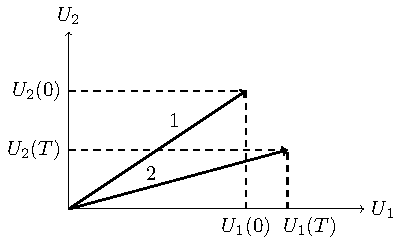
\includegraphics[width=0.35\linewidth]{fig/fig41.pdf}   
\end{figure}

По переменной $U_1$ увеличение вектора, по $U_2$ - уменьшение. Процесс повторяется. Вектор вытягивается и прижимается к оси абсцисс. Если $n\rightarrow \infty$ (число итераций): $U_2(nT)\rightarrow 0,~U_1(nT)\rightarrow \infty$. В системе реализуется параметрический параметрический резонанс. 

Получим приближенное соотношение для $x_1(t)$:
\begin{gather*}
	\lambda_1=\frac{1}{T}ln(s_1)>0, \\
	\lambda_2=\frac{1}{T}ln(s_2)=\frac{1}{T}ln(\frac{1}{s_1})=-\frac{1}{T}ln(s_1)<0.
\end{gather*}

Функция Флоке ограниченная
\begin{equation*}
	x_1(t)\approx c_1 e^{\frac{1}{T}ln(s_1)t}\Phi_{11}(t).
\end{equation*}
\begin{figure}[H]
	\centering
	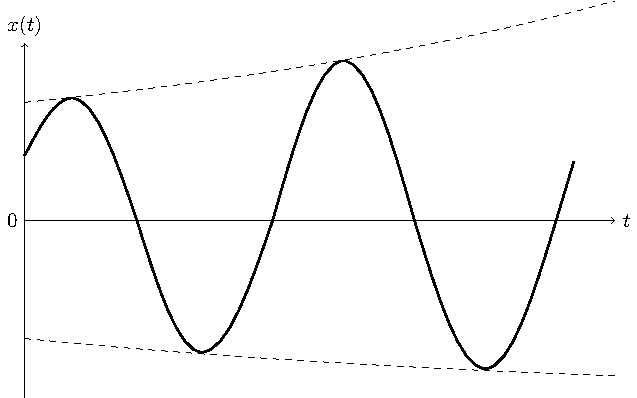
\includegraphics[width=0.5\linewidth]{fig/fig42.pdf}   
\end{figure}

В начальный момент система должна быть выведена из равновесия. Это геометрическая прогрессия, экстремумы функции лежат на экспоненте. 
\begin{itemize}
	\item В линейном осцилляторе экстремумы на прямых;
	\item Если линейный осциллятор в покое, мы можем его раскачать;
\end{itemize}

Пусть $s_1,s_2<0,~|s_1|>1,~|s_2|<1$:
\begin{figure}[H]
	\centering
	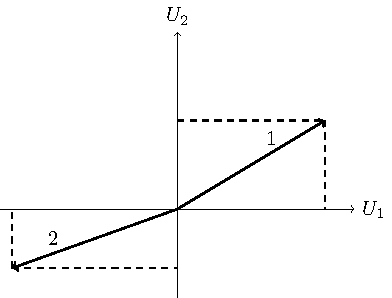
\includegraphics[width=0.5\linewidth]{fig/fig43.pdf}   
\end{figure}

Вектор вернется через 2 итерации, период 2T, экстремумы отстоят на период.
\begin{figure}[H]
	\centering
	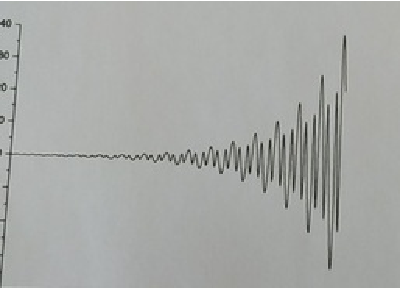
\includegraphics[width=0.4\linewidth]{fig/fig44.pdf}   
\end{figure}

Пусть $|P|=1$. В этом случае, если $P=1$, то $s_1=s_2=1$; если $P=-1$, то $s_1=s_2=-1$. Корни кратные, мы такое не рассматривали. Решение в этом случае задается в виде:
\begin{gather*}
	x_1(t)=c_1 e^{\lambda t}\Phi(t)+c_2te^{\lambda t}\Phi(t), \\
	\lambda=\frac{1}{T}ln|s|.
\end{gather*}

На границе неустойчивость и состояние равновесия $x_1=x_2=0$ является неустойчивым.

\subsection{Параметрические колебания маятника}
\begin{equation}
	\ddot{\varphi}+2\delta \dot{\varphi}+\frac{g}{l(t)}\varphi=0.
	\label{eq:81}
\end{equation}

Рассмотрим маятник, у которого длина периодически меняется, $\delta$ характеризует диссипацию. Кусочно-линейная аппроксимация. $l(t+T)=l(t)$.

Будем считать, длина меняется мгновенно:
\begin{equation*}
	l(t)=
	\left\{\begin{aligned}
		l_0-\frac{a}{2}, 0 \leq t \leq \frac{T}{2} \\
		l_0+\frac{a}{2}, \frac{T}{2} \leq t \leq T		
	\end{aligned}\right.
\end{equation*}

далее периодично. Получается меандр.
\begin{equation*}
	l_0=\frac{a}{2}>0,~\omega_1^2=\frac{g}{l_0-\frac{a}{2}},~\omega_2^2=\frac{g}{l_0+\frac{a}{2}}.
\end{equation*}

Рассмотрим консервативный случай ($\delta=0$). Перепишем \eqref{eq:81} в виде:
\begin{equation}
	\left\{\begin{aligned}
		\dot{\varphi}=y \\
		\dot{y} =-\omega^2(t)\varphi.	
	\end{aligned}\right.
	\label{eq:82}
\end{equation}
\begin{equation}
	\omega^2(t)=
	\left\{\begin{aligned}
		\omega^2_1, 0 \leq t \leq \frac{T}{2} \\
		\omega^2_2, \frac{T}{2} \leq t \leq T		
	\end{aligned}\right.
	\label{eq:83}	
\end{equation}

\eqref{eq:82} является частным случаем рассмотренного выше, где $p_{21}=\omega^2(t)$. Для построения областей надо построить границы $P=\pm 1$, найдя a,d. Они являются элементами матрицы G. которая задает $g^T$. Поскольку система является кусочно-линейной, можно представить: $G=G_1\cdot G_2$, где $G_1$ действует на интервале от 0 до $\frac{T}{2}$, $G_2$ от $\frac{T}{2}$ до $T$. 

\underline{Матрица $G_1$:}

$\omega^2(t)\equiv\omega_1^2$

Решая \eqref{eq:82}:
\begin{gather*}
	\varphi_1(t)\equiv A_1 \cos(\omega_1 t) + B_1\sin(\omega_1 t), \\
	\varphi_2(t)\equiv -A_1 \sin(\omega_1 t) + \omega_1 B_1\cos(\omega_1 t).
\end{gather*}

Положим: $\varphi_1(0)=1,~\varphi_2(0)=0$. $A_1=1,~B_1=0$. Искомое решение примет вид: 
\begin{equation}
	\left\{\begin{aligned}
		\varphi_1(t) = \cos(\omega_1 t) \\
		\varphi_2(t) = -\sin(\omega_1 t).		
	\end{aligned}\right.
	\label{eq:84}	
\end{equation}

Аналогично находится второе решение:
\begin{gather}
	\psi_1(0)=0, \psi_2(0)=1, \notag \\
	\left\{\begin{aligned}
		\psi_1(t) = \frac{\sin(\omega_1 t)}{\omega_1} \\
		\psi_2(t) = \cos(\omega_1 t).		
	\end{aligned}\right.
	\label{eq:85}	
\end{gather}

Подставляя $t=\frac{T}{2}$, найдем элементы $G_1$:
\begin{equation}
	\left\{\begin{aligned}
		a_1 = \cos(\omega_1 \frac{T}{2}) \\
		b_1 = -\omega_1 \sin(\omega_1 \frac{T}{2}) \\
		c_1 = \frac{\sin(\omega_1 \frac{T}{2})}{\omega_1} \\
		d_1 = \cos(\omega_1 \frac{T}{2}),	
	\end{aligned}\right.
	\label{eq:86}	
\end{equation}
\begin{gather*}
	G_1= 
	\begin{pmatrix}
		\cos \alpha~~~~~\frac{\sin\alpha}{\omega_1} \\
		-\omega_1 \sin \alpha~~\cos \alpha
	\end{pmatrix}
	, 
	\alpha=\omega_1 \frac{T}{2}.	
\end{gather*}

\underline{Матрица $G_2$:}
Вид устанавливается аналогично:
\begin{gather*}
	G_1= 
	\begin{pmatrix}
		\cos \beta~~~~~\frac{\sin\beta}{\omega_2} \\
		-\omega_2 \sin \beta~~\cos \beta
	\end{pmatrix}
	, 
	\beta=\omega_2 \frac{T}{2}.	
\end{gather*}

\underline{ $G_1\cdot G_2$:}

Получили матрицу, элементы которой имеют вид:
\begin{gather*}
	a=\cos \alpha \cdot \cos \beta -\frac{\omega_1}{\omega_2} \sin \alpha \cdot \sin \beta, \\
	b=-\omega_2 \cos \alpha \cdot \sin \beta - \omega_1 \sin \alpha \cdot \sin \beta, \\
	c=\frac{\sin \alpha \cdot \cos \beta}{\omega_1}+\frac{\cos \alpha \cdot \sin \beta}{\omega_2}, \\
	d=\cos \alpha \cdot \cos \beta-\frac{\omega_2}{\omega_1}\sin \alpha \cdot \sin \beta,
\end{gather*}
\begin{equation}
	2P=a+d=2\cos \alpha\cdot \cos \beta - \frac{\omega_1^2+\omega_2^2}{\omega_2 \omega_1} \sin \alpha \cdot \sin \beta.
	\label{eq:87}	
\end{equation}

Введем более физичные параметры: собственная частота, если бы длина не менялась: $\omega_0^2=g/l_0$; период, если бы длина не менялась: $T_0=2\pi /\omega_0$; глубина параметрической модуляции: $\varepsilon=a/2l_0$; отношение собственного периода к периоду параметрической накачки: $\gamma=T/T_0$. Тогда:
\begin{gather*}
	\alpha=\frac{\pi \gamma}{\sqrt{1-\epsilon}},~\beta=\frac{\pi \gamma}{\sqrt{1+\epsilon}},~\frac{\omega_1^2+\omega_2^2}{\omega_2 \omega_1}=\frac{2}{\sqrt{1-\epsilon^2}},~\varepsilon<1.
\end{gather*}

Если $\varepsilon=0$, то параметрической модуляции нет.
\begin{equation}
	P=\cos(\frac{\pi \gamma}{\sqrt{1-\epsilon}}) \cos (\frac{\pi \gamma}{\sqrt{1+\epsilon}}) - \frac{1}{\sqrt{1-\epsilon^2}} \sin(\frac{\pi \gamma}{\sqrt{1-\epsilon}}) \sin (\frac{\pi \gamma}{\sqrt{1+\epsilon}}).
	\label{eq:88}	
\end{equation}

20.05

Таким образом, у нас осталось два параметра: $\gamma$ и $\varepsilon$. Строим границы, где реализуется параметрический резонанс, используя формулу \eqref{eq:88}. Подставим в \eqref{eq:88} $\varepsilon=0$. P примет вид: $P=\cos(2\pi \gamma)$.

Границы области: $P=\pm1, P=0$.
\begin{gather*}
	P=0 \rightarrow	\gamma=\frac14+\frac{k}2,~k=0,1,2,\dots, \\
	P=-1 \rightarrow	\gamma=k+\frac12,~k=0,1,2,\dots, \\
	P=1 \rightarrow	\gamma=k,~k=1,2,\dots.
\end{gather*}

Нарисуем плоскость параметров (для малых $\varepsilon$, построен численно; при увеличении $\varepsilon$ границы зоны сближаются, образуют петлю и снова расходятся):
\begin{figure}[H]
	\centering
	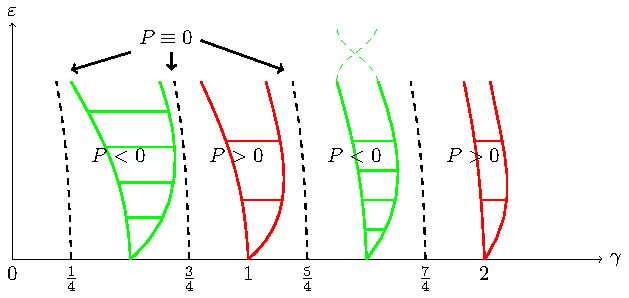
\includegraphics[width=0.5\linewidth]{fig/fig45.pdf}   
\end{figure}

Получились "клювы", выходящие из последовательности точек на оси абсцисс. Таких точек бесконечное число. 

Зоны становятся уже с увеличением номера. Одно семейство образует $P^-$ зоны, лежащие в области $P<0$. Семейство в $P^+$ лежат в других областях. Во всех зонах реализуется параметрическая неустойчивость. В зонах, принадлежащих $P^-$ мультипликаторы нулевого состояния равновесия являются отрицательными, в $P^+$ - положительными.  

Вне этих зон будут либо периодические, либо квазипериодические колебания, в зависимости от параметра $\gamma$. Диссипация, если таковая имеется, приведет к тому, что глубины модуляции изменятся. Зоны будут начинаться не с 0, а с $\varepsilon>0$. 